\documentclass[12pt,fleqn]{article}
\setlength{\parindent}{0pt}
\usepackage{graphicx}
\usepackage{cancel}
\usepackage{listings}
\usepackage[latin5]{inputenc}
\setlength{\parskip}{8pt}
\setlength{\parsep}{0pt}
\setlength{\headsep}{0pt}
\setlength{\topskip}{0pt}
\setlength{\topmargin}{0pt}
\setlength{\topsep}{0pt}
\setlength{\partopsep}{0pt}
\setlength{\mathindent}{0cm}

\begin{document}
MIT OCW Cok Degiskenli Calculus - Ders 15

Onceki derslerde gradyan kavramini gorduk. Bu vektorun bilesenleri, 3
degiskenli bir fonksiyon icin

\[ \nabla f = <f_x, f_y, f_z> \]

idi, ki bu bilesenler $f$'in tum kismi turevlerini
olusturuyordu. Gradyanlar kismi turevleri paketlemenin, sunmanin
yontemlerinden biriydi sadece. 

Gradyanlari yaklasiksallama formulleri icin de kullanabiliyorduk, mesela
eger $x,y,z$'yi ``birazcik'' degistirince bunun $f$ uzerindeki degisim
etkisi $\Delta f$'i [kabaca, niye kabaca oldugu altta] hesaplamak
istiyorsak bunun gradyan formundaki hali

\[ \Delta f \approx f_x \Delta x + f_y \Delta y + f_z \Delta z \]

Daha kisa olarak 

\[ = \nabla f \cdot \Delta \vec{r} \]

oluyordu, yani gradyan vektorunun, pozisyon vektorunun degisimi ile olan
noktasal carpimi. Kismi turevlerin tami tamina olctugu sey $f$'in bir
degiskendeki degisime ne kadar hassas oldugudur, ve bu hassasligin ufak
degisimler ile carpilip toplanmasi bize tum fonksiyondaki degisimi verir.

Ustteki yaklasiksallama ``teget duzlem yaklasiksallamasi'' olarak bilinir,
bu arada, fonksiyonun yerine bir noktada teget duzlemi koyuyoruz, o noktada
fonksiyon budur diyoruz, boylece fonksiyonun $x,y,z$ degiskenlerine asagi
yukari lineer olarak bagli oldugunu farz ediyoruz, o sebeple zaten
degisimleri duz carpim sonrasi basit toplama maruz tutuyoruz. 

Hatirlarsak, $f(x,y,z)=c$ yuzeyine teget olan duzlemi bulmak icin normal
vektore bakariz, biliyoruz ki normal vektorlerden biri fonksiyonun gradyan
vektorudur, cunku gradyanin kesit seviyelerine diktir, ve fonksiyonun daha
yuksek degerlerine, en yuksek artis yonune isaret etmektedir. 

Bu noktada kulturel bir not eklemek istiyorum. Bunu belki haftalar once
belirtmeliydim, daha iyi olurdu. Kismi turevleri niye seviyoruz /
kullaniyoruz? Onemli bir sebep onlarin fizik icin cok faydali olmalari,
etrafimizdaki dunyayi anlamamiza yardimci olmalari. Bu dunyadaki pek cok
olus kismi turevsel denklemler (partial differential equations -PDE-) ile
tarif edilir, modellenir.

PDE'ler bilinmeyen bir fonksiyonun kismi turevlerini kullanarak onlar
arasinda bir iliski, fonksiyon kurar. 

Mesela Isi Denklemi (Heat Equation) bunlardan biridir. 

\[ \frac{\partial f}{\partial t}  = k (
\frac{\partial^2 f}{\partial x^2} + 
\frac{\partial^2 f}{\partial y^2} + 
\frac{\partial^2 f}{\partial z^2} )
\]

Bu denklemde cozmek, bulmak istedigimiz $f$ fonksiyonudur, ve bu
fonksiyon 4 degiskene baglidir: $f(x,y,z,t)$, ve temsil ettigi $x,y,z$
pozisyonundaki bir noktanin $t$ anindaki sicakligidir. PDE
$\partial f/\partial t$ ise bu fonksiyonun zamana gore nasil degistigini
tarif eder. 

Bu konuya ileride tekrar donecegiz. 

Simdi diger konulara gecelim. Kritik noktalardan bahsetmistik, bu
noktalarda kismi turevler sifir degerlerindeydi. Ayrica eger noktalari
(saddle points) vardi, ve ikinci turevleri kullanarak kritik noktanin min
mi, maks mi, eger mi  olduguna karar verebiliyorduk. 

Fakat tum bunlarin min, maks bulmak icin yeterli olmadigini da gorduk,
cunku min, maks sinir noktalarinda, fonksiyonun ta en uclarinda da
olabiliyordu. 

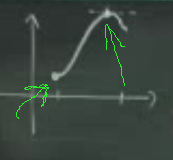
\includegraphics[height=4cm]{15_1.png}

Ustteki grafikte gorulen sagdaki nokta kritik bir nokta, ve ikinci turevin
bize lokal maks oldugunu soyleyecegi noktadir. Minimum ise soldaki
noktadir, fonksiyonun sol sinirindadir, ve kritik nokta degildir. Birden
fazla degisken icin de durum aynidir; bu durumlarda min, maks bulmak icin
degiskenlerin olabilecekleri en az degere (mesela sifir) ya da en fazla
(mesela sonsuzluk) cekmek gerekebilir. Yani zihnimizi acik tutup pek cok
olasiligi gozden gecirmemiz, dusunmemiz gerekir. 

Diferansiyeller 

$f$'teki degisimi soyle gosterdik

\[ df = f_xdx + f_ydy + f_zdz  \]

Ilk bakista bu temsil, kismi turevleri paketlemenin bir baska yolundan
ibaret gozukuyor. Bunu da yapiyor muhakkak, ama daha fazlasi da
var. Yaklasiksal formullerin formunu hatirlamanin iyi bir yolu, her
degiskendeki varyasyonu digerlerinkiyle ilintilendiriyoruz. Bir onemli
fayda daha su, bu formulu ayni $d\_$ ile bolerek, degisik sekillerdeki
Zincirleme Kanunlarini ortaya cikarabiliriz. 

Mesela diyelim ki $x,y,z$ diger iki degisken $u,v$'ye bagli. 

\[ x = x(u,v) \]

\[ y = y(u,v) \]

\[ z = z(u,v) \]

Bu durumda $f$, aslinda $u,v$'nin bir fonksiyonu haline gelir. Ve bu
noktada kendimize $f$ fonksiyonu mesela ``$u$'nun degisimine ne kadar
hassas'' gibi bir soru sorabiliriz. Bunun cevabini Zincirleme Kanununu $u$
uzerinden kullanarak cevaplayabiliriz. 

\[ 
\frac{\partial f}{\partial u} = 
\frac{\partial f}{\partial x}\frac{\partial x}{\partial u} + 
\frac{\partial f}{\partial y}\frac{\partial y}{\partial u} + 
\frac{\partial f}{\partial z}\frac{\partial z}{\partial u} 
 \]

Ustteki turde bir islem bize degisken degisimi yaptigimiz zaman faydali
olur. Mesela kutupsal kordinat sisteminden $x,y$ kordinat sistemine gecis
yapabiliriz, ve Zincirleme Kanunu uzerinden kutupsal formdaki degisimin $x,y$
dunyasindaki yansimalarini hesaplayabiliriz. 

Sonraki konumuz bagimsiz olmayan degiskenler, mesela $x,y,z$, degiskenleri
$g(x,y,z)=c$ gibi bir fonksiyon uzerinden birbiriyle baglantili. Her
seferinde bu tur problemlerde istedigimiz degiskeni yanliz birakip, baska
bir yerlere koyamiyoruz, o zaman min, maks baglaminda Lagrange Carpanlari
teknigini kullaniyoruz.

Bir diger gordugumuz teknik kisitlanmis kismi turevler teknigiydi. Diyelim
ki yine elimizde $f(x,y,z)$ var ve $g(x,y,z)=c$ gibi bir baglanti var. Bu
durumda $f$'in tek bir degisken degisip, digerleri sabit iken (yani tipik
kismi turev islemi) nasil degisecegini bulabilir miyim? 

Bulamayabilirim, cunku, belki kisitlama ibaresi $g$ yuzunden geri kalan tum
degiskenleri sabit tutamayacagim.

Ornek 

Sunu bul

\[ 
\bigg( 
\frac{\partial f}{\partial z}
\bigg)_{y}
 \]

$y$ sabit

$z$ degisiyor

\[ x = x(y,z) \]

Ustteki $x$ ibaresini bu ornek icin biz tanimladik, herhangi baska bir
kisitlama ibaresi $g$ olabilirdi. 

1) Diferansiyelleri Kullanarak

Genel ifade neydi?
\[ df = f_xdx + f_ydy + f_zdz \]  

Bunu ozel durumumuza nasil uygulariz? $y$ sabit, o zaman $dy = 0$. Yani

\begin{equation}\label{eq1}
df = f_xdx + f_zdz  
\end{equation}

Devam edelim, aslinda $dx$'den de kurtulmak istiyoruz, cunku o bagimli bir
degisken, her seyi $z$ formunda gormek istiyoruz. Bunun icin once $dg$'yi
bulalim. 

\[ dg = g_xdx + g_ydy + g_zdz = 0   \]

Niye sifira esit? Cunku $g$ kisitlama ibaresi sabitti. 

$y$ degismiyorsa, o zaman ustteki $dy$ de gidebilir. Kalanlar

\[ dg = g_xdx + g_zdz = 0  \]

\[ dx = -\frac{g_z}{g_x}dz \]

Yani 

\[ 
\bigg( \frac{\partial x}{\partial z}\bigg)_{y} = -\frac{g_z}{g_x}
 \]

O zaman iki ustteki formulu alip, \ref{eq1}. formulde $dx$ yerine 
koyarsak

\[ df = (-f_x\frac{g_z}{g_x} +  f_z) dz \]








\end{document}
